%&mybeamer
%\documentclass[ignoreonframetext,12pt]{beamer}
%\documentclass{mybeamer}

% Meta data
\author{Daniel Hoske}
\title{Book Embedding with Fixed Page Assignments}
\date{23rd October 2012}
\institute{Department of Informatics, Institute of Theoretical Computer Science\\
Advisors: Dipl.-Inform. Thomas Bläsius, Dr. Ignaz Rutter}


\newcommand{\SEFE}{\prob{sefe}}
\newcommand{\SEFECON}{\prob{connected-sefe}}
\newcommand{\PQ}{PQ\xspace}
\newcommand{\Q}{Q\xspace}
\newcommand{\PT}{P\xspace}

% Algorithmic problems
\newcommand{\prob}[1]{\textsc{#1}\xspace}
\newcommand{\probTwoSat}{\prob{2-sat}}
\newcommand{\probThreeSat}{\prob{3-sat}}
\newcommand{\probQTree}{\prob{q-tree-book-embedding}}
\newcommand{\probPTree}{\prob{p-tree-book-embedding}}
\newcommand{\probQTreeSat}{\prob{q-tree-2-sat}}
\newcommand{\probBookNormal}{\prob{not-fixed-book-embedding}}
\newcommand{\probBook}{\prob{book-embedding}}
\newcommand{\probBookConnected}{\prob{connected-book-embedding}}
\newcommand{\probBetween}{\prob{betweenness}}
\newcommand{\probBookOrder}{\prob{order-book-embedding}}
\newcommand{\probMatching}{\prob{perfect-matchings-book-embedding}}
\newcommand{\probNotMatching}{\prob{matchings-book-embedding}}
\newcommand{\probPQ}{\prob{simultaneous-pq-ordering}}
\newcommand{\probMul}{\prob{multiple-spine-embedding}}
\newcommand{\probThreeMatching}{\prob{3-perfect-matchings-book-embedding}}
\newcommand{\range}[1]{\{1, \dotsc, #1\}}
\newcommand{\newProb}[3]{%

\vspace{.5em}
\begin{block}{Problem: #1}
\emph{Given:} #2\\%
%\emph{Answer the question:} #3%
\emph{Question:} #3%
\end{block}
\vspace{.5em}
}    

% Tikz options
\tikzstyle{dashdot} = [dash pattern=on .8pt off 3pt on 4pt off 3pt]
\tikzstyle{edge1}=[red,dashed]
\tikzstyle{edge2}=[blue,dotted]
\tikzstyle{edge3}=[green,dashdot]
\tikzstyle{every node}+=[inner sep=0.5mm,minimum size=2.00mm,node distance=3em,thick]
\tikzstyle{every edge}+=[thick]
\tikzstyle{every arc}+=[thick]
\tikzstyle{every path}+=[thick]
\usetikzlibrary{svg.path,calc,decorations.pathreplacing,positioning,backgrounds}
\newdimen\XCoord
\newdimen\YCoord
\newcommand*{\ExtractCoordinate}[1]{\path #1; \pgfgetlastxy{\XCoord}{\YCoord};}%

\newcommand{\drawedges}[2][\empty]{
	\foreach \a/\b in {#2}{
		\draw[#1] (\a) edge (\b);
	}
}

% Semicircle through a and b
\newcommand{\semicircle}[2]{%
  \ExtractCoordinate{($ 0.5*($ (#2.north) - (#1.north) $) $)}
  \draw[thick] ($ (#2.north) $) arc (0:180:\XCoord);
}

\def\caption[#1]#2{}

\newcommand{\mytt}[1]{{\footnotesize \texttt{#1}}}

\newcommand{\solutionTri}[2]{
  \begin{figure}\centering
  \resizebox{#2}{!}{
  \begin{tikzpicture}
    \coordinate (1) at (0,0);
    \coordinate (2) at (60:8);
    \coordinate (3) at (8,0);
    
	\draw (1) -- (2)
	      (2) -- (3)
	      (3) -- (1);    
    
    \node (centre) at ($ 1/3*($ (1) + (2) + (3) $) $) {3 pages?};    
    
    \ifthenelse{#1 > 0}{\node (a) at ($ (2) + (0, .5) $) {$2$ pages: $\OO(n)$};}{}
    \ifthenelse{#1 > 1}{\node (b) at ($ (1) + (0, -.5)$) {$k$ connected pages: $\OO(kn)$};}{
                        \node[white] (b) at ($ (1) + (0, -.5)$) {$k$ connected pages: $\OO(kn)$};}
    \ifthenelse{#1 > 2}{\node (c) at ($ (3) + (0, -.5) $) {$k$ matchings: in NPC};}{}
    \ifthenelse{#1 > 3}{\node (d) at ($ 0.5*($ (3) + (centre) $) + (-.5,0) $) {$3$ perfect matchings?};}{}
    \ifthenelse{#1 > 4}{
      \node (e) at ($ (1) + (0,-1) $) {P-trees?};
      \node (f) at ($ (e) + (3,0) $) {Q-trees: $\OO(kn^2)$};
      \draw (e) -- (f);
    }{}
    
    \draw[draw=none, use as bounding box](-2,-2) rectangle (10,8);
  \end{tikzpicture}
  }
  \end{figure}
}

\newcommand{\resultFrame}[1]{
  \miniframesoff
  \begin{frame}{Results}
    \solutionTri{#1}{0.8\textwidth}
  \end{frame}
  \miniframeson
}

\begin{document}

\miniframesoff
\setbeamerfont{title}{size=\large}
\setbeamerfont{author}{size=\normalsize}
%\setbeamerfont{institute}{size=\normalsize}
\begin{frame}\titlepage\end{frame}

\begin{frame}{Page embedding}
\begin{definition}
\emph{Page embedding} is planar embedding with\\
      \begin{itemize}
        \item vertices on a line and
        \item edges in half-plane above the line
      \end{itemize}
\end{definition}

\begin{overprint}
\onslide<1>
\begin{figure}
\centering

\scalebox{0.5}{\begin{tikzpicture}

\draw[->,thin] (-1em,0) -- ++(9em, 0) node [right] {x};
\draw[->,thin] (-1em,0) -- ++(0,9em)  node [above] {y};

\node[fill=white] (1) {a};
\node[fill=white,right of=1] (2) {b};
\node[fill=white,right of=2] (3) {c};

\draw (1) edge [bend left] (2);
\draw (2) edge [bend left] (3);
\draw (1) edge [bend left] (3);
\end{tikzpicture}}

\end{figure}
Page embeddable = outerplanar
\onslide<2>
Page embeddable = outerplanar
\begin{figure}\centering
\resizebox{0.7\textwidth}{!}{
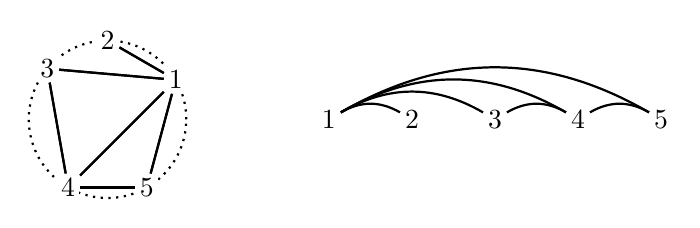
\begin{tikzpicture}
    \tikzstyle{every node}+=[fill=white]
	\draw[dotted] (0, 0) circle (1);
	\node (1) at (30:1) {1};
    \node (2) at (90:1) {2};
	\node (3) at (140:1) {3};
	\node (4) at (240:1) {4};
	\node (5) at (300:1) {5};
	\drawedges{1/2,3/4,1/3,1/4,1/5,4/5};
	\draw (1) -- (2);
	\draw (3) -- (4);
	\draw (1) -- (3);
	\draw (1) -- (4);
	\draw (1) -- (5);
	\draw (4) -- (5);
	
    \node[draw=none,fill=none] at (2.0,0) {{\Huge $\rightsquigarrow$}};	
	
	\begin{scope}[xshift=8em]
	\node (1) at (0, 0) {1};
	\node (2) [right of=1]{2};
    \node (3) [right of=2]{3};
	\node (4) [right of=3]{4};
	\node (5) [right of=4]{5};
    \drawedges[bend left]{1/2,3/4,1/3,1/4,1/5,4/5};		
	\end{scope}
\end{tikzpicture}
}
\end{figure}
\end{overprint}
\end{frame}

\begin{frame}{Book embedding}

\begin{definition}
\emph{Book embedding} of $G_i = (V, E_i)$, $i \in \range{k}$ consists of 
page embeddings for~$G_i$ with the same vertex positions.
\end{definition}

\begin{overprint}
\onslide<1>
\begin{figure}
\centering

\resizebox{0.6\textwidth}{!}{
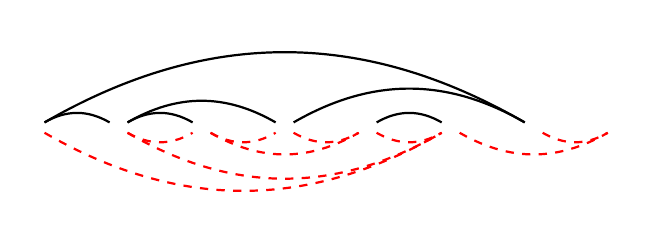
\begin{tikzpicture}
\node (1) {};
\node [right of=1] (2) {};
\node [right of=2] (3) {};
\node [right of=3] (4) {};
\node [right of=4] (5) {};
\node [right of=5] (6) {};
\node [right of=6] (7) {};
\node [right of=7] (8) {};

\drawedges[bend left]{1/2,2/4,2/3,1/7,5/6,4/7}
\drawedges[bend right,edge1]{2/3,3/4,2/6,3/5,4/5,5/6,6/8,7/8,1/6}
\end{tikzpicture}}
\end{figure}

\onslide<2>

\newProb{\probBook}{Vertex set $V$ and edge sets $E_1,\dotsc, E_k \subseteq \binom{V}{2}$.}
{Is there a book embedding of $(V, E_i)$?}
$k = 1$: embeddable = outerplanar\\
$k = 2$: decidable in $\OO(n)$ [Hong and Nagamochi, 2009]\\
What happens for $k = 3$?
\end{overprint}
\end{frame}

\begin{frame}{Motivation}
\newProb{\SEFECON\label{prob:sefecon}}{Two graphs~$G_1$ and~$G_2$ on~$V$ where~$G_1 \cap G_2$ is connected.}{Are 
there planar embeddings of~$G_1$ and~$G_2$ that coincide on~$G_1 \cap G_2$?}

is equivalent to 2-page book embedding + a tree [Angelini et al., 2012]
\begin{tabular}{m{0.3\textwidth}m{0.7\textwidth}}
  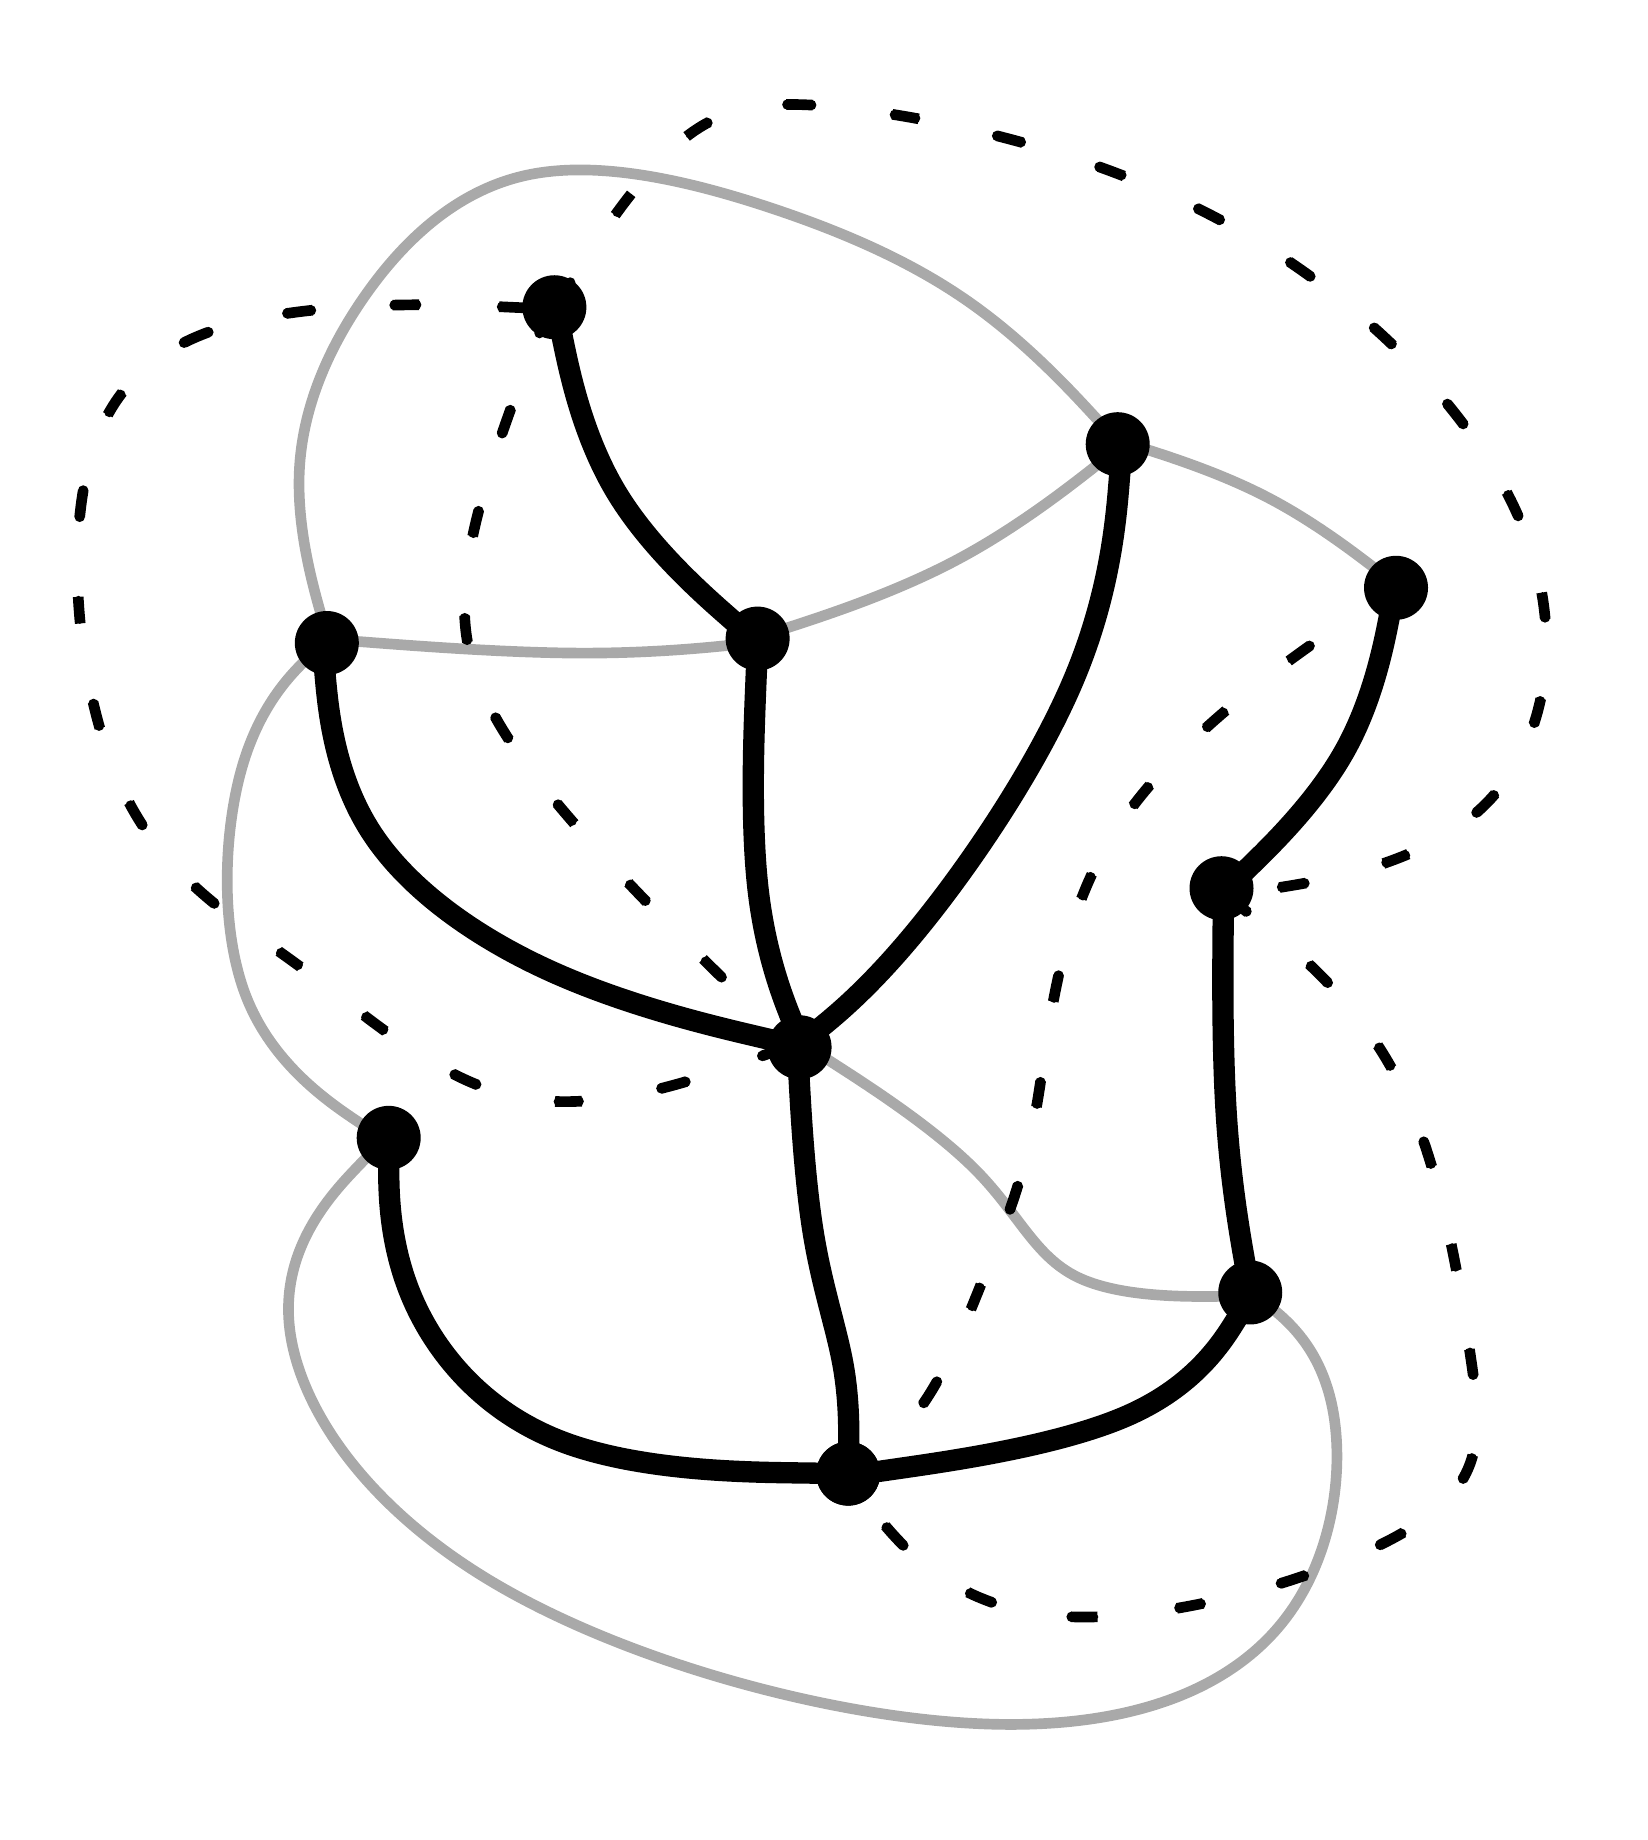
\includegraphics[width=0.3\textwidth]{sefe1} &
  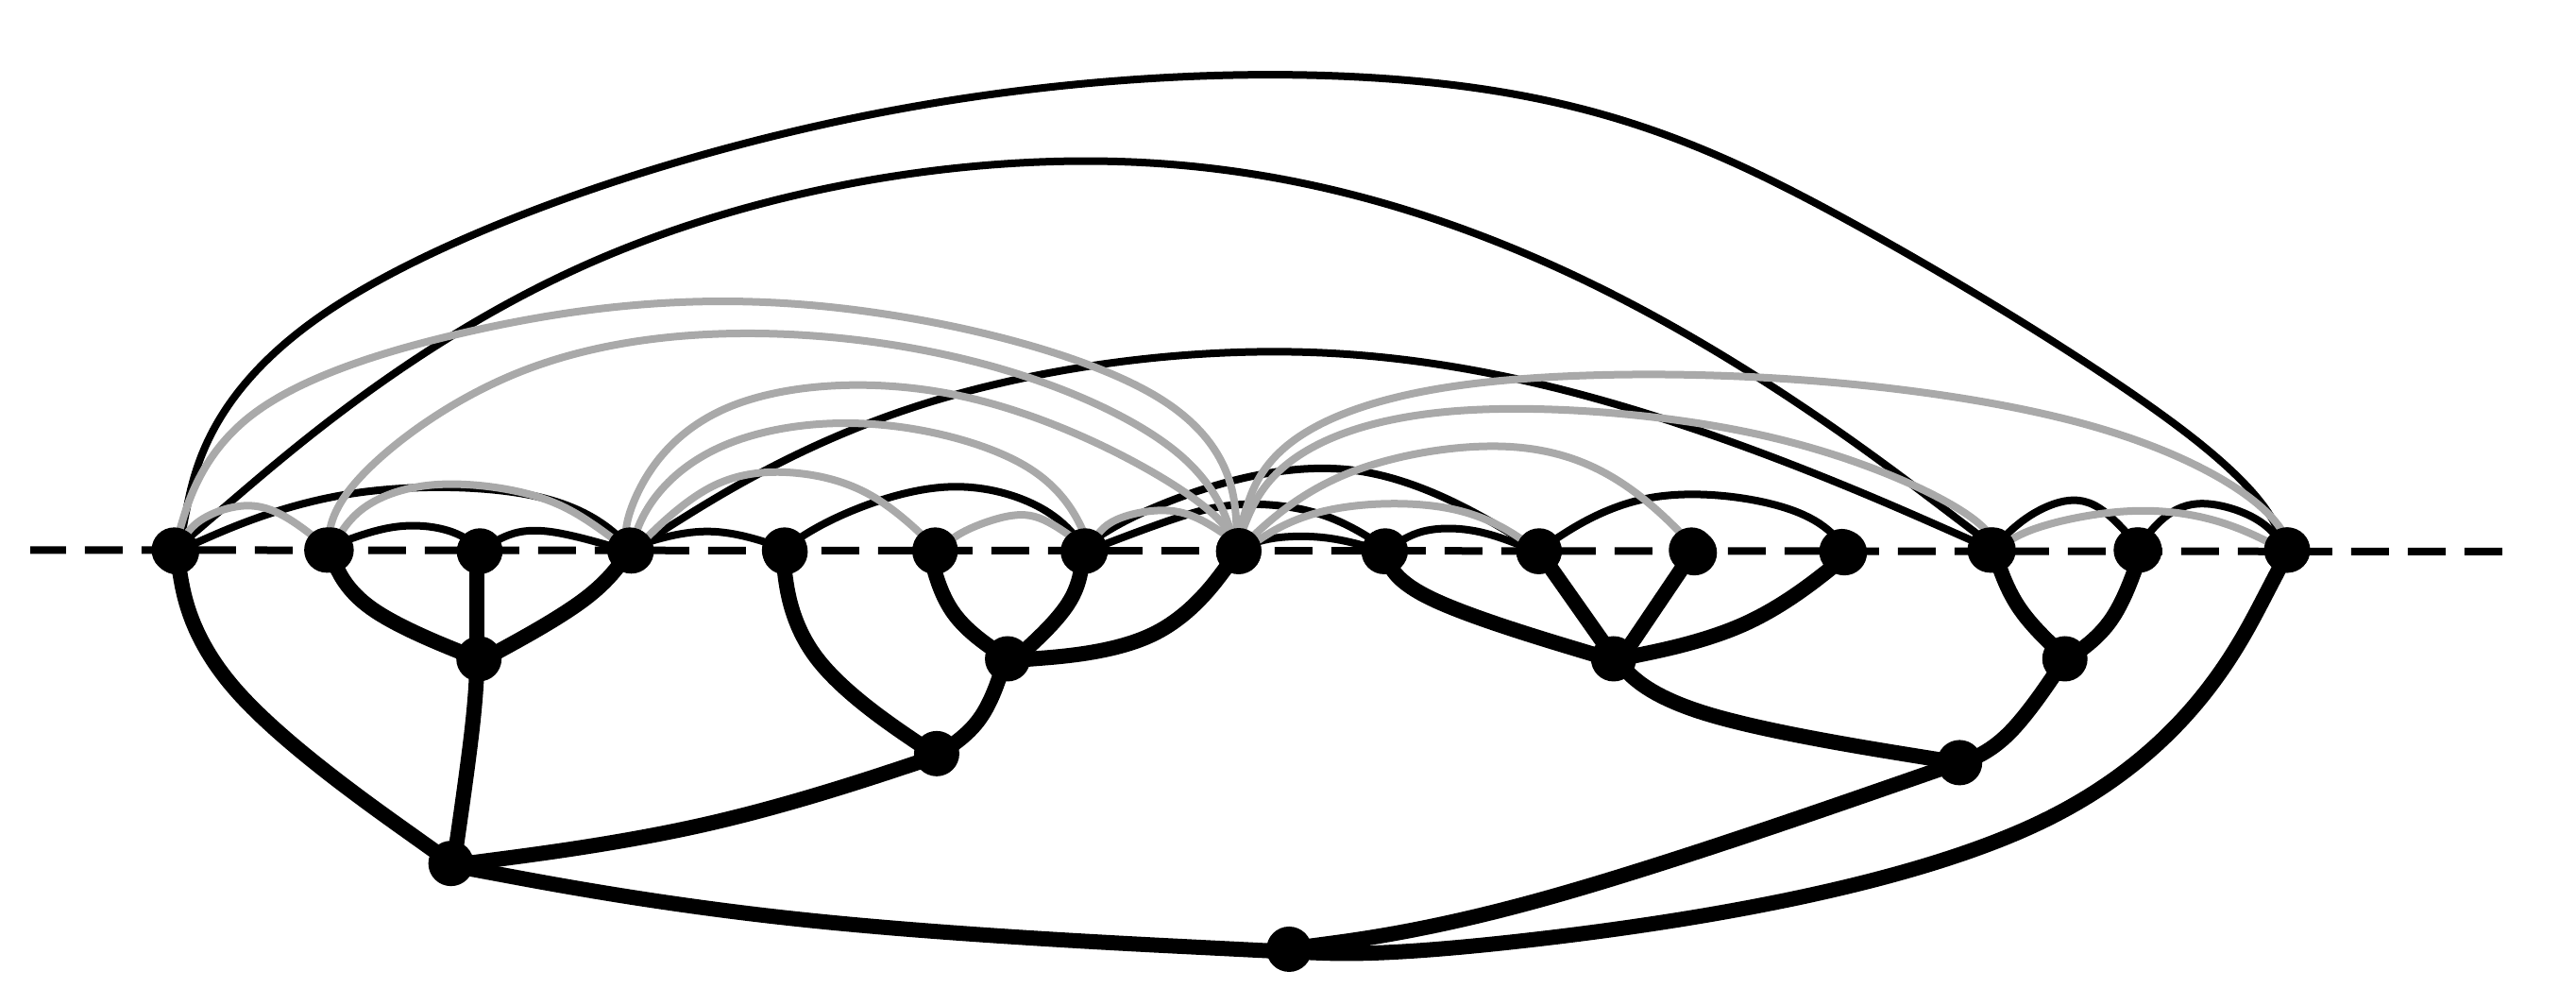
\includegraphics[width=0.65\textwidth]{sefe2}
\end{tabular}
\end{frame}

%\begin{frame}{\PQ-trees}
%\begin{definition}
%A \emph{\PQ-tree} $T$~on $M := \range{n}$ is a rooted, ordered
%tree with leaves~$M$ and inner nodes either of type~$P$ (\tikz[scale=0.4,baseline={([yshift=+0.1em]current bounding box.south)}] \draw (0,0) circle (1em);)
%or type~$Q$ (\tikz[scale=0.75,baseline={([yshift=+0.1em]current bounding box.south)}] \draw (-0.5em, -0.5em) -- ++(1em, 0) -- ++(0, 1em) -- ++ (-1em,0) -- ++(0,-1em);).
%\\[1em]
%The order of the children
%of a \PT-node can be permuted in any way, while the order of the children of a \Q-node can only be reversed. The tree represents the set of permutations~$\pi(T) \subseteq \Sym(M)$ that consists exactly of the permutations of the leaves~$M$ that we can get
%by flipping the inner nodes in any of the specified valid ways.
%\end{definition}
%\end{frame}

\begin{frame}{Observations}
  \probBook is an ordering problem:\\
  Avoid suborder $a < c < b < d$ for $\{a, b\}, \{c, d\} \in E_i$

\begin{figure}[\placement]
\centering

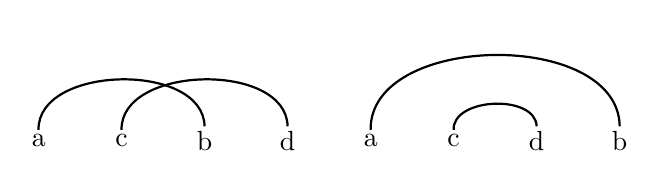
\begin{tikzpicture}
\node (a) {a};
\node [right of=a] (c) {c};
\node [right of=c] (b) {b};
\node [right of=b] (d) {d};

\drawedges[bend left,out=90,in=90]{a/b,c/d}

\begin{scope}[xshift=12em]
\node (a) {a};
\node [right of=a] (c) {c};
\node [right of=c] (d) {d};
\node [right of=d] (b) {b};

\drawedges[bend left,out=90,in=90]{a/b,c/d}
\end{scope}
\end{tikzpicture}
\end{figure}

Mirror image and cyclic shifts of a valid order remain valid:

\begin{figure}[\placement]
\centering

\resizebox{\textwidth}{!}{%
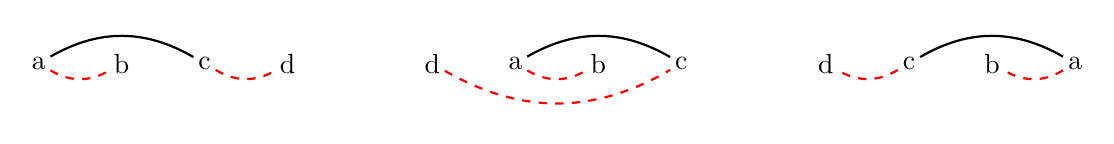
\begin{tikzpicture}
\begin{scope}
\node (a) {a};
\node [right of=a] (b) {b};
\node [right of=b] (c) {c};
\node [right of=c] (d) {d};

\draw (a) edge [bend left] (c);

\draw[edge1] (a) edge [bend right] (b);
\draw[edge1] (c) edge [bend right] (d);
\end{scope}

\begin{scope}[xshift=5cm]
\node (d) {d};
\node [right of=d] (a) {a};
\node [right of=a] (b) {b};
\node [right of=b] (c) {c};

\draw (a) edge [bend left] (c);
\draw[edge1] (a) edge [bend right] (b);
\draw[edge1] (d) edge [bend right] (c);
\end{scope}

\begin{scope}[xshift=10cm]
\node (d) {d};
\node [right of=d] (c) {c};
\node [right of=c] (b) {b};
\node [right of=b] (a) {a};

\draw (a) edge [bend right] (c);

\draw[edge1] (a) edge [bend left] (b);
\draw[edge1] (c) edge [bend left] (d);

\end{scope}
\end{tikzpicture}}
\end{figure}
\end{frame}

\resultFrame{1}

\begin{frame}
\frametitle{Contents}
\tableofcontents
\end{frame}

\miniframeson

%\section{Basic observations}

\begin{frame}{Total order formulation}
  Book embedding instance is solvable if and only if\\there is a total order~$<$ on~$V$ (\emph{valid order})
  without suborder \[a < c < b < d\] 
  for $\{a, b\}, \{c, d\} \in E_i$ (\emph{book constraint}).

\begin{figure}[\placement]
\centering

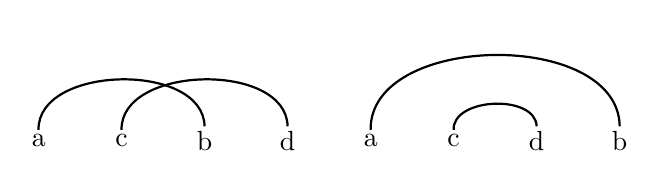
\begin{tikzpicture}
\node (a) {a};
\node [right of=a] (c) {c};
\node [right of=c] (b) {b};
\node [right of=b] (d) {d};

\drawedges[bend left,out=90,in=90]{a/b,c/d}

\begin{scope}[xshift=12em]
\node (a) {a};
\node [right of=a] (c) {c};
\node [right of=c] (d) {d};
\node [right of=d] (b) {b};

\drawedges[bend left,out=90,in=90]{a/b,c/d}
\end{scope}
\end{tikzpicture}

\end{figure}
\end{frame}

\begin{frame}{Valid orders}

Mirror image and cyclic shifts of valid order are valid:

\begin{figure}[\placement]
\centering

\resizebox{\textwidth}{!}{%
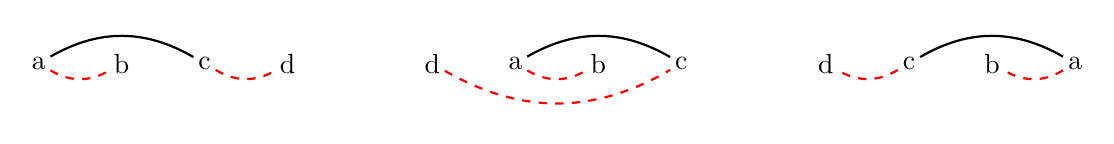
\begin{tikzpicture}
\begin{scope}
\node (a) {a};
\node [right of=a] (b) {b};
\node [right of=b] (c) {c};
\node [right of=c] (d) {d};

\draw (a) edge [bend left] (c);

\draw[edge1] (a) edge [bend right] (b);
\draw[edge1] (c) edge [bend right] (d);
\end{scope}

\begin{scope}[xshift=5cm]
\node (d) {d};
\node [right of=d] (a) {a};
\node [right of=a] (b) {b};
\node [right of=b] (c) {c};

\draw (a) edge [bend left] (c);
\draw[edge1] (a) edge [bend right] (b);
\draw[edge1] (d) edge [bend right] (c);
\end{scope}

\begin{scope}[xshift=10cm]
\node (d) {d};
\node [right of=d] (c) {c};
\node [right of=c] (b) {b};
\node [right of=b] (a) {a};

\draw (a) edge [bend right] (c);

\draw[edge1] (a) edge [bend left] (b);
\draw[edge1] (c) edge [bend left] (d);

\end{scope}
\end{tikzpicture}}

\end{figure}
\end{frame}

\section{\NP-completeness and connected pages}

\begin{frame}{\probBook is \NP-complete}

\begin{theorem}
\probBook with matchings as pages is \NP-complete.
\end{theorem}

Reduce from \NP-complete problem \probBetween [Opatrny, 1979].
\newProb{\probBetween}{Finite set $M := \range{n}$ and ordered triples $C \subseteq M^3$.}
{Is there a total ordering $<$ of $M$ such that $a < b < c$ or $a > b > c$ for all $(a, b, c) \in C$?}
\end{frame}

\begin{frame}{Reduction from \probBetween}

\newProb{\probBetween}{Finite set $M := \range{n}$ and ordered triples $C \subseteq M^3$.}
{Is there a total ordering $<$ of $M$ such that $a < b < c$ or $a > b > c$ for all $(a, b, c) \in C$?}

Map triple~$(a, b, c) \in C$ to two new pages ($r$ fixed new vertex):	
\begin{figure}
\centering

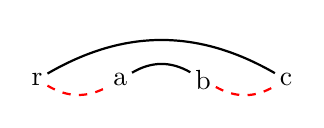
\begin{tikzpicture}
% a < b < c
\node (r) {r};
\node [right of=r] (a) {a};
\node [right of=a] (b) {b};
\node [right of=b] (c) {c};

\draw[edge1] (r) edge [bend right] (a);
\draw[edge1] (b) edge [bend right] (c);
\draw (a) edge [bend left]  (b);
\draw (r) edge [bend left]  (c);  
\end{tikzpicture}

\end{figure}

\begin{overprint}
\onslide<1>
For example: $(a, b, c)$, $(b, c, d)$
\begin{figure}\centering
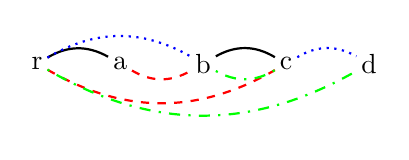
\begin{tikzpicture}
% a < b < c
\node (r) {r};
\node [right of=r] (a) {a};
\node [right of=a] (b) {b};
\node [right of=b] (c) {c};
\node [right of=c] (d) {d};

\drawedges[bend left]{r/a,b/c};
\drawedges[bend left,edge2]{r/b,c/d};
\drawedges[bend right,edge1]{a/b,r/c};
\drawedges[bend right,edge3]{b/c,r/d};
\end{tikzpicture}
\end{figure}

\onslide<2>
\probBetween $\Rightarrow$ \probBook:\\
Take~$r$ as first vertex\\
$\rightsquigarrow$ Orders $r < a < b < c$ or $r < c < b < a$ are valid

\onslide<3>
\probBook $\Rightarrow$ \probBetween:\\
Rotate $r$ to front\\
$\rightsquigarrow$ $r < a < b < c$ or $r < c < b < a$ are the only valid orders

\end{overprint}
\end{frame}



\begin{frame}<1>[label=connected,fragile]{Connected pages}

\begin{theorem}
\probBook with connected pages can be solved in $\OO(kn)$~time.
\end{theorem}

\begin{overprint}
\onslide<1>
Idea:\\Compute valid orders $\pi_i \subseteq \Sym(n)$ for single pages and\\intersect them.

\begin{figure}\centering
\resizebox{0.3\textwidth}{!}{
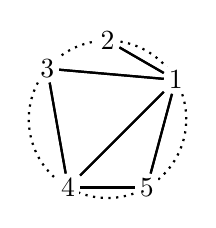
\begin{tikzpicture}
    \tikzstyle{every node}+=[fill=white]
	\draw[dotted] (0, 0) circle (1);
	\node (1) at (30:1) {1};
    \node (2) at (90:1) {2};
	\node (3) at (140:1) {3};
	\node (4) at (240:1) {4};
	\node (5) at (300:1) {5};
	\drawedges{1/2,3/4,1/3,1/4,1/5,4/5};
	\draw (1) -- (2);
	\draw (3) -- (4);
	\draw (1) -- (3);
	\draw (1) -- (4);
	\draw (1) -- (5);
	\draw (4) -- (5);
\end{tikzpicture}
}
\end{figure}

\onslide<2>

\begin{itemize}
\item Construct \PQ-trees $T_i$ on~$V$ representing valid orders of individual pages
$(V,E_i)$
\begin{figure}
\centering
\resizebox{0.6\textwidth}{!}{
\begin{tikzpicture}
\path[use as bounding box] (-2,2) rectangle (8,-2.5);

\tikzstyle{every node}+=[minimum size=0.5cm,thick]
\tikzstyle{every path}+=[thick]

\node[] (a) {$a$};
\node[right of=a] (b) {$b$};
\node[below of=b] (c) {$c$};
\node[left of=c] (d) {$d$};
\node[left of=a, above of=a] (r) {$r$};

\draw (a) edge (b) 
      (b) edge (c) 
      (c) edge (d) 
      (d) edge (a);
\draw[dashed] (r) edge (a)
              (r) edge (b)
              (r) edge (d)
              (r) edge[out=270, in=270, min distance=6em] (c);

% PQ-tree
\begin{scope}[xshift=5cm]
\node[draw,rectangle,minimum size=.2cm] {}
   child {node {$a$}}
   child {node {$b$}}
   child {node {$c$}}
   child {node {$d$}};
\end{scope}
\end{tikzpicture}}
\end{figure}

[Booth and Lueker et. al. 1976, Shih and Hsu 1993,\\Boyer and Myrvold 1999]
\end{itemize}

\onslide<3>
\begin{itemize}
\item Construct \PQ-trees $T_i$ on~$V$ representing valid orders of individual pages
$(V,E_i)$
\item Intersect the $T_i$ [Booth, 1975]
\item[$\rightarrow$] Resulting \PQ-tree~$T$ represents valid book orders
\end{itemize}
\end{overprint}

\end{frame} 

\begin{frame}{Interludium: \PQ-trees}

\begin{overprint}
\onslide<1>
$\hspace{4em}T = 
\begin{aligned}
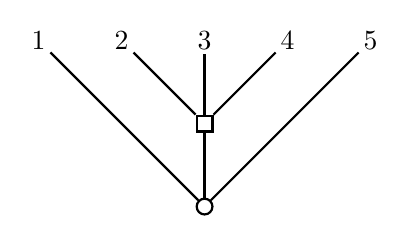
\begin{tikzpicture}

\tikzstyle{every path}+=[thick]

\node (1) {1};
\node[right of=1] (2) {2};
\node[right of=2] (3) {3};
\node[right of=3] (4) {4};
\node[right of=4] (5) {5};

\node[rectangle, draw, below of=3] (t2) {};
\node[circle, draw, below of=t2] (t1) {};

\draw (t1) edge (1);
\draw (t1) edge (5);
\draw (t2) edge (2);
\draw (t2) edge (3);
\draw (t2) edge (4);
\draw (t1) edge (t2);
\end{tikzpicture}
\end{aligned}$

\onslide<2>
$\hspace{4em}T = 
\begin{aligned}
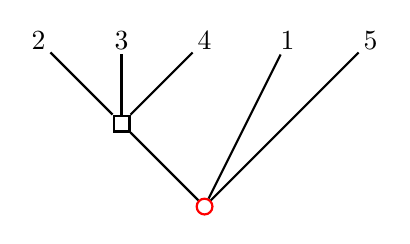
\begin{tikzpicture}

\tikzstyle{every path}+=[thick]

\node (2) {2};
\node[right of=2] (3) {3};
\node[right of=3] (4) {4};
\node[right of=4] (1) {1};
\node[right of=1] (5) {5};

\node[rectangle, draw, below of=3] (t2) {};
\node[circle, draw, below of=t2,right of=t2,red] (t1) {};

\draw (t1) edge (1);
\draw (t1) edge (5);
\draw (t2) edge (2);
\draw (t2) edge (3);
\draw (t2) edge (4);
\draw (t1) edge (t2);
\end{tikzpicture}
\end{aligned}$

\onslide<3>
$\hspace{4em}T = 
\begin{aligned}
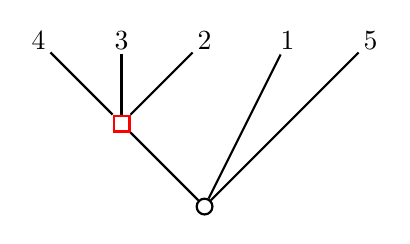
\begin{tikzpicture}

\tikzstyle{every path}+=[thick]

\node (4) {4};
\node[right of=4] (3) {3};
\node[right of=3] (2) {2};
\node[right of=2] (1) {1};
\node[right of=1] (5) {5};

\node[rectangle, draw, below of=3,red] (t2) {};
\node[circle, draw, below of=t2,right of=t2] (t1) {};

\draw (t1) edge (1);
\draw (t1) edge (5);
\draw (t2) edge (2);
\draw (t2) edge (3);
\draw (t2) edge (4);
\draw (t1) edge (t2);
\end{tikzpicture}
\end{aligned}$
\end{overprint}

\begin{align*}
\pi(T) & = \{\only<1>{\alert{12345}}\only<2->{12345}, 14325, 52341, 54321, 15234, 15432, \\
         & \hspace{1.8em} 51234, 51432, \only<2>{\alert{23415}}\only<1,3->{23415}, \only<3>{\alert{43215}}\only<1-2>{43215}, 23451, 43251\}
\end{align*}
\end{frame}

\againframe{connected}

\resultFrame{3}
%\section{Connected Graphs}\label{section:connected}

One approach for solving the book embedding problem is to
determine the
set of valid total orders (permutations) for each of the pages and obtain
the valid book orders by intersecting these sets. Since there are~$n!$ 
permutations on~$n$ vertices, this method is not efficient and even needs super-polynomial space. Indeed, we have
shown in the previous chapter that we cannot expect there to be an efficient algorithm.

We know that cyclic shifts and mirror images do not matter. Considering this, 
we can encode the possible valid orders more efficiently by 
only storing one symmetric order in place of $2n$ total orders. However, this
is still not sufficient for efficiently solving the book embedding problem.
Are there better encodings that make the algorithm
feasible, at least for special graphs?

As a matter of fact, there are. In this section we see that the valid total orders can be encoded
very efficiently using \PQ-trees if the pages are connected---the first special case of~\probBook we consider. Furthermore, \PQ-trees on the
same vertices can also be efficiently \emph{intersected}, \ie we can efficiently 
get a \PQ-tree representing~$\pi(T_1) \cap \pi(T_2)$ from two \PQ-trees $T_1$ and~$T_2$ on the same leaves.

\newProb{\probBookConnected}{A vertex set~$V$ and edge sets~$E_1,\dotsc,E_k \subseteq \binom{V}{2}$ such
that the graphs~$(V, E_i)$ are connected for~$i \in \range{k}$.}{Is there
a book embedding of $(V, E_1),\dotsc, (V,E_k)$?}

%TODO
%
%We can reinterpret a \PQ-tree to represent a set of cyclic orders instead of linear order.
%To do this, add a new root $p$~whose only neighbour is the original root of the tree. In all possibilities
%for flipping the tree's \PT- and \Q-nodes, define the corresponding circular order as follows: Start at~$p$, go along the
%linear order of the tree and end at~$p$. If we disregard~$p$ in this order, we get a circular order on
%the original leaves. That is, we can map a linear order on the
%leaves to a cyclic order by
%writing the leaves in the linear order on a cycle.
%Since, for example, 12345 and~23451 both yield the
%same cyclic order, this map need not be injective.

\paragraph{Planarity testing using \PQ-trees}

There are several planarity testing algorithms that represent the possible planar
embeddings using \PQ-trees. A high-level scheme for these methods is
described by Haeupler and Tarjan~\cite{Haeupler08}. It can be adapted to give
all valid orders of a page embedding as we show below.

We first briefly describe this scheme. 
It embeds the graph $G$~vertex by vertex. At each step
we store the set of possible partial planar embeddings where some subset
of the vertices has already been embedded. 

The edges that have exactly 
one embedded endpoint at a step are \emph{half-embedded}. If the non-embedded
vertices form a connected graph at each step, the half-embedded edges must lie on a common face
that we can without loss of generality assume to be the outer face, \ie all the already embedded vertices incident to half-embedded edges are on the boundary of the outer face. 

That the non-embedded vertices form a connected graph can be guaranteed
by choosing a leaf-to-root order in any fixed spanning tree of the connected graph~$G$. The possible
partial embeddings can then be represented by the order of their half-embedded edges
around the outside of their component.
 
It can be shown that these orders are given by a \PQ-tree for every component of the subgraph
induced by the embedded vertices. For a more detailed explanation consult the
paper by Haeupler and Tarjan~\cite{Haeupler08}. They also show how to implement the
scheme in linear time.

\paragraph{Representing book embeddings using \PQ-trees}

This is not yet what we want. A page embedding is an outerplanar embedding and not a planar embedding.
Thus, we have to modify the planarity algorithm slightly. We build the connected graph $\widetilde{G}$ by
adding a new vertex~$r$ to~$G$ that is adjacent to every vertex in~$V(G)$. In \myref{ch:preliminaries} we noted the
fact that~$G$ is outerplanar if and only if $\widetilde{G}$ is planar. Furthermore, by removing~$r$
from a planar embedding of~$\widetilde{G}$ we get an outerplanar embedding of~$G$.

\begin{figure}[\placement]
    \centering
    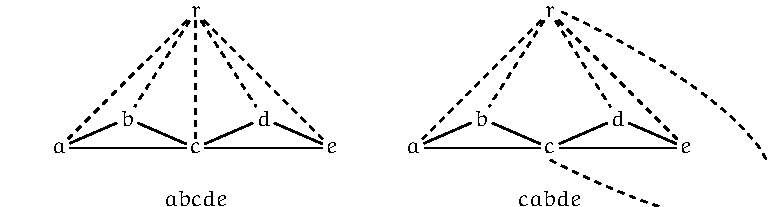
\includegraphics[scale=.9]{figures/t_subtle}
    \caption[Outerplanar embedding representing different symmetric orders]{The outerplanar embedding  
    represents the vertex orders in both $[abcde]$ and~$[cabde]$. The symmetric orders $[abcde]$ and~$[cabde]$ correspond to different edge orders around~$r$ in the extended graph.}
    \label{figure:subtle}
\end{figure}
    
Now we choose~$r$ as last vertex in the leaf-to-root order of the planarity algorithm.
Since $G$~is connected, the scheme above yields a single \PQ-tree~$T$ representing all
extendible planar embeddings of~$G$ (as possible orders of the half-embedded edges~$\{r, v\}$ for~$v\in V(G)$)  at its penultimate step. By the argument above, every such embedding
is outerplanar. Also, $T$~not only gives the orders of the half-embedded edges
but all vertices of~$G$ since~$r$ is adjacent to every other vertex, \ie every vertex of~$G$ is 
the endpoint of exactly one half-embedded edge. 

A subtle distinction is still noteworthy, although it does not present any problems
for the algorithm. When
walking around the outer boundary of an outerplanar embedding in clockwise or counter-clockwise
direction, we can meet a vertex twice. Thus, the outerplanar embedding in \myref{figure:subtle},
for example, can yield the total orders in both $[abcde]$ and~$[cabde]$; yet these orders belong
to different planar embeddings of the extended graph.

In conclusion, there is a \PQ-tree from which we can read all valid outerplanar embeddings (page embeddings). 
This \PQ-tree can be computed in linear time as shown by Haeupler and Tarjan~\cite{Haeupler08}.
%For~$C_4$ this is illustrated in \myref{figure:connected}.

\begin{lemma}\label{lemma:one-page}
Let~$G = (V, E)$ be a connected graph. Then we can compute a \PQ-tree representing all valid
orders of the vertices~$V$ in a page embedding of~$G$ in $\OO\bigl(|V|\bigr)$~time.
\end{lemma}

To get the set of valid book orders, all that remains to be done is to intersect the
\PQ-trees we get. Say we want to intersect the \PQ-trees~$S$ and~$T$ on the same leaves. Let~$v$
be an inner node of~$S$ and~$e$ one of its incident edges going to a child~$w$ of~$v$.
Then the leaves $C(w)$~that have~$w$ as ancestor appear consecutively in any order $\pi \in \pi(S)$.
Additionally, if~$v$ is a \Q-node and $e'$ is a consecutive edge of~$e$ going from~$v$ to~$w'$, then the
leaves $C(w) \cup C(w')$ also appear consecutively in any $\pi \in \pi(S)$. On the other hand,
any order fulfilling these constraints is in~$\pi(S)$. That is, we can get a tree
representing $\pi(S) \cap \pi(T)$ by applying the reductions just described to the tree~$T$.
A trivial implementation of this approach would need a quadratic number of reductions, but Booth described in his Ph.\,D. thesis~\cite{Booth75}
how to reduce the cost of intersection to linear time.

Now that we are able to intersect \PQ-trees, we can summarise the linear-time solution
of \probBookConnected.

\begin{theorem}
\probBookConnected can be solved in linear time.
\label{theorem:connected}
\end{theorem}
\begin{myproof}
Let~$(V, E_1,\dotsc, E_k)$ be the \probBookConnected instance.
First construct the $k$ \PQ-trees~$T_1,\dotsc, T_k$ representing all valid page
embeddings of the corresponding graphs~$(V, E_1), \dotsc, (V,E_k)$, each in~$\OO\bigl(|V|\bigr)$. Then consecutively
intersect $T_1$ with $T_2,\dotsc, T_k$ using time~$\OO\bigl((k - 1)|V|\bigr)$, yielding the
\PQ-tree~$T$ representing all valid solutions of the instance. The instance
possesses a solution if and only if~$T \ne \varepsilon$, which can be decided in constant time.
All in all, we need $\OO\bigl(k|V|\bigr)$~time.
\end{myproof}

\paragraph{Outlook}

When the graphs on the pages are not connected, we also get \PQ-trees for the valid orders of each of their components. That is, we have a set of \PQ-trees and must decide whether
they possess a common order in order to solve the book embedding problem. The hurdle is that the trees do not need to have the same leaves. 

Bl\"asius and Rutter~\cite{Blasius11} considered a more general variant of this \PQ-tree intersection problem, called \probPQ. They showed the
\NP-completeness of \probPQ for an unbounded number of trees. 
%As noted in \myref{section:np-complete}, we, similarly, only showed that \probBook
%is \NP-complete when the number of pages is unbounded. 
Investigating restrictions of \probPQ
may help us deal with the book embedding problem, but we are not sure how.
%By the reduction above, we can
%improve this to a constant number of pages if we manage to prove the \NP-completeness
%of \probPQ for a constant number of trees. Therefore, investigating \probPQ is one approach for extending
%our results, but it is---in our opinion---not promising since
%\probPQ is not a problem of significantly simpler form than \probBook.
\section{Disjoint perfect matchings}

\begin{frame}{Disjoint perfect matchings as pages}

%Take disjoint perfect matchings as pages.
\newProb{\probMatching}
{Disjoint perfect matchings $E_1,\dotsc, E_k$ on a vertex
set $V$.}{Is there a book embedding of $(V, E_i)$?}

\begin{theorem}
Necessary: $G := (V, E_1 \cup \dotsb \cup E_k)$ is bipartite.
\end{theorem}

\begin{overprint}
\onslide<1>
\begin{itemize}
\item Even number of vertices between adjacent vertices in valid order
\begin{figure}
\centering

\resizebox{0.6\textwidth}{!}{
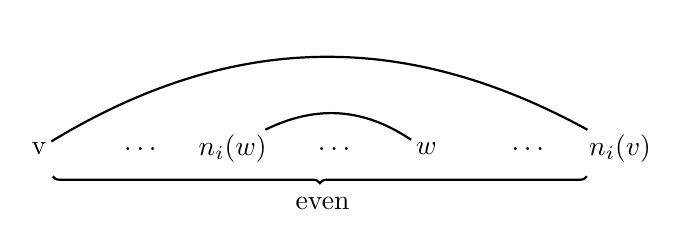
\begin{tikzpicture}
\node (v) {v};
\node[right of=v,node distance=7em] (nw) {$n_i(w)$};
\node[right of=nw,node distance=7em] (w) {$w$};
\node[right of=w,node distance=7em] (nv) {$n_i(v)$};

\draw (v) edge[bend left] (nv);
\draw (nw) edge[bend left] (w);

/* v to n1 */
\draw[decoration={brace},decorate,thick] ($ (nv) + (-1.2em, -1em) $) -- ($ (v) + (0.5em,-1em) $);
\node[text centered] at ($ 0.5*($(nv) + (v)$) + (-0.25em, -2em) $) {even};

\node[text centered] at ($ 0.5*($(v) + (nw)$) + (0.25em, 0)$) {\dots};
\node[text centered] at ($ 0.5*($(nw) + (w)$) + (0.25em, 0)$) {\dots};
\node[text centered] at ($ 0.5*($(w) + (nv)$) + (0.25em, 0)$) {\dots};
\end{tikzpicture}
}
\end{figure}
\end{itemize}

\onslide<2>
\begin{itemize}
\item Even number of vertices between adjacent vertices in valid order
\item[$\Rightarrow$] Vertices with even and odd indexes form bipartition
\end{itemize}
\end{overprint}

\end{frame}

\begin{frame}{Bipartite examples}
\begin{figure}[\placement]
\centering

\scalebox{1.3}{%
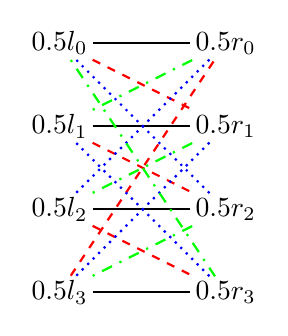
\begin{tikzpicture}

\node (l1) {{\relscale{0.5}$l_0$}};
\node[right of=l1,node distance=6em] (r1) {{\relscale{0.5}$r_0$}};
\node[below of=l1] (l2) {{\relscale{0.5}$l_1$}};
\node[right of=l2,node distance=6em] (r2) {{\relscale{0.5}$r_1$}};
\node[below of=l2] (l3) {{\relscale{0.5}$l_2$}};
\node[right of=l3,node distance=6em] (r3) {{\relscale{0.5}$r_2$}};
\node[below of=l3] (l4) {{\relscale{0.5}$l_3$}};
\node[right of=l4,node distance=6em] (r4) {{\relscale{0.5}$r_3$}};

\draw (l1) edge (r1);
\draw (l2) edge (r2);
\draw (l3) edge (r3);
\draw (l4) edge (r4);
\draw[edge1] (l1) edge (r2);
\draw[edge1] (l2) edge (r3);
\draw[edge1] (l3) edge (r4);
\draw[edge1] (l4) edge (r1);
\draw[edge2] (l1) edge (r3);
\draw[edge2] (l2) edge (r4);
\draw[edge2] (l3) edge (r1);
\draw[edge2] (l4) edge (r2);
\draw[edge3] (l1) edge (r4);
\draw[edge3] (l2) edge (r1);
\draw[edge3] (l3) edge (r2);
\draw[edge3] (l4) edge (r3);
\end{tikzpicture}}
\end{figure}

$k$ pages: Take the partition $E_i := \bigl\{\{l_j, r_{(j + i)\bmod{k}}\}: j \in \range{k-1}\bigr\}$ of $K_{k,k}$ 
\end{frame}

\begin{frame}{Bipartite counterexamples}
\begin{figure}[\placement]
\centering

\scalebox{1.3}{%
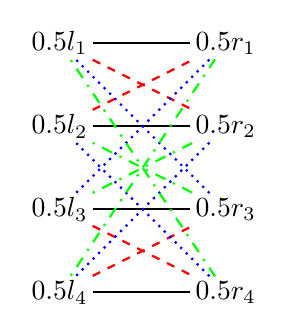
\begin{tikzpicture}

\node (l1) {{\relscale{0.5}$l_1$}};
\node[right of=l1,node distance=6em] (r1) {{\relscale{0.5}$r_1$}};
\node[below of=l1] (l2) {{\relscale{0.5}$l_2$}};
\node[right of=l2,node distance=6em] (r2) {{\relscale{0.5}$r_2$}};
\node[below of=l2] (l3) {{\relscale{0.5}$l_3$}};
\node[right of=l3,node distance=6em] (r3) {{\relscale{0.5}$r_3$}};
\node[below of=l3] (l4) {{\relscale{0.5}$l_4$}};
\node[right of=l4,node distance=6em] (r4) {{\relscale{0.5}$r_4$}};

\draw (l1) edge (r1);
\draw (l2) edge (r2);
\draw (l3) edge (r3);
\draw (l4) edge (r4);
\draw[edge1] (l1) edge (r2);
\draw[edge1] (l2) edge (r1);
\draw[edge1] (l3) edge (r4);
\draw[edge1] (l4) edge (r3);
\draw[edge2] (l1) edge (r3);
\draw[edge2] (l3) edge (r1);
\draw[edge2] (l2) edge (r4);
\draw[edge2] (l4) edge (r2);
\draw[edge3] (l1) edge (r4);
\draw[edge3] (l4) edge (r1);
\draw[edge3] (l2) edge (r3);
\draw[edge3] (l3) edge (r2);
\end{tikzpicture}}
\end{figure}

$k \geq 4$ pages: Partition $K_{k,k}$ into disjoint perfect matchings that contain
this counterexample
\end{frame}

\begin{frame}{Bipartite counterexample for three pages}
Smallest counterexample where two of the matchings form a cycle\vspace{-1em}
\begin{figure}[\placement]
\centering
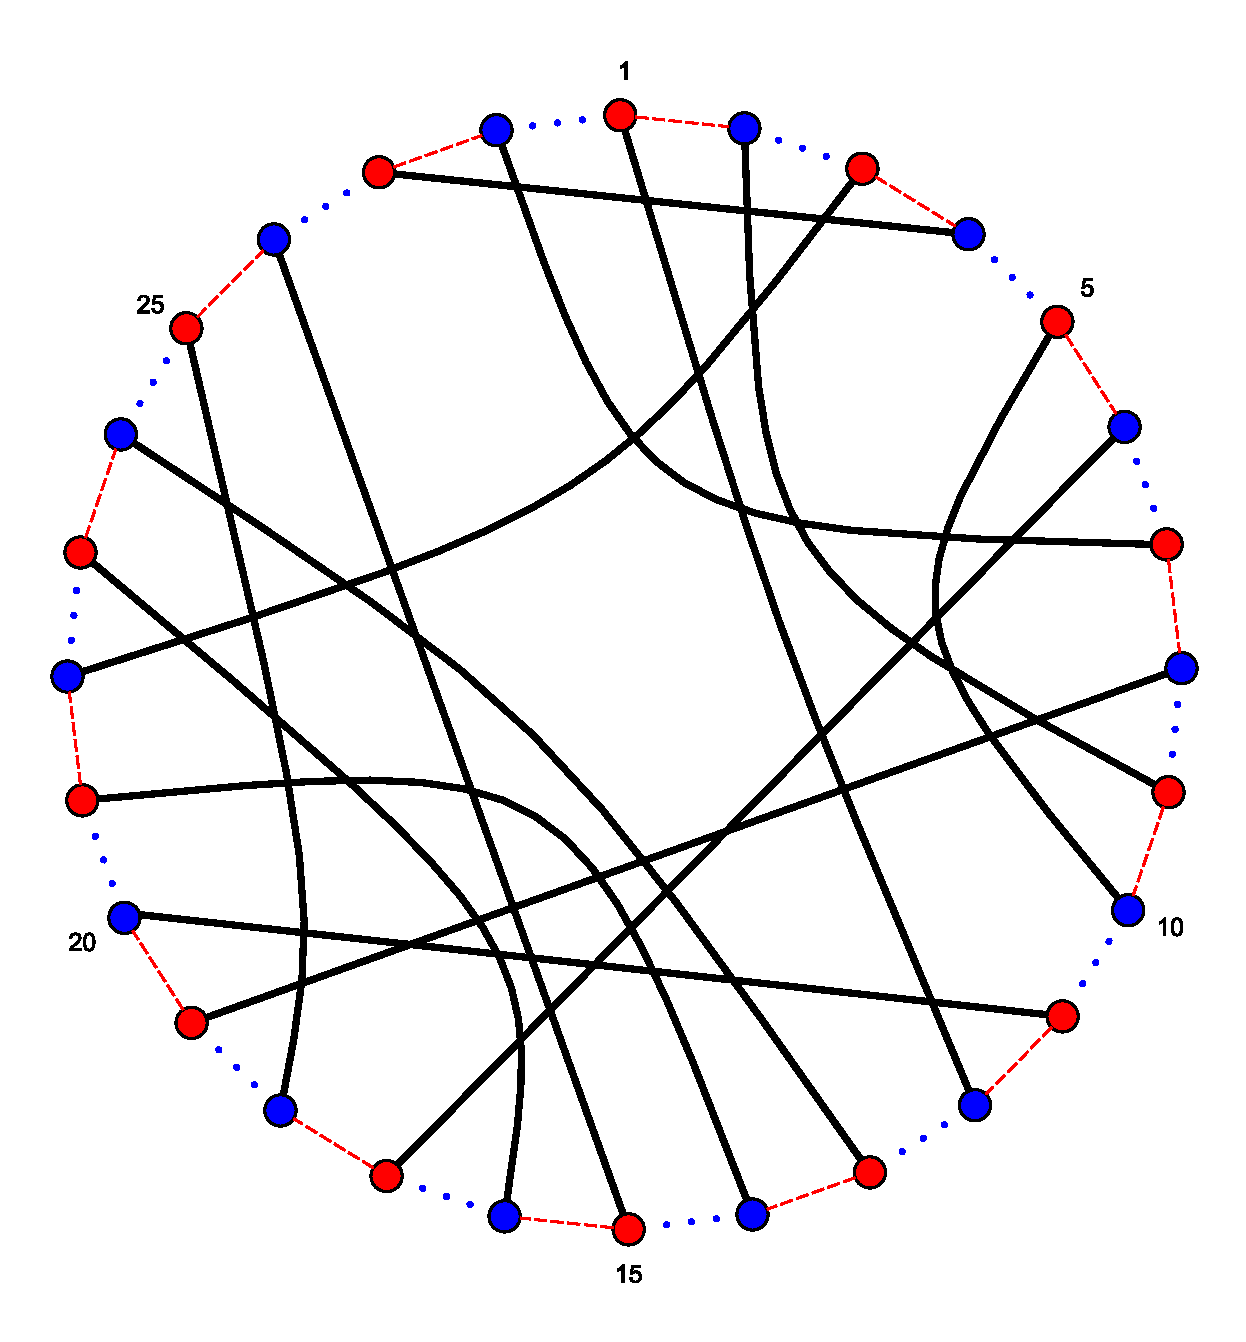
\includegraphics[width=0.5\textwidth]{../thesis/figures/two_cycles.eps}
\end{figure}
\vspace{-1em} Smallest unrestricted counterexample: $20 \leq n \leq 28$
\end{frame}

\resultFrame{4}
\section{Tree on the vertices}

\begin{frame}{Tree on the vertices}

\probBook + tree:

\begin{overprint}
\onslide<1>
\begin{figure}\centering
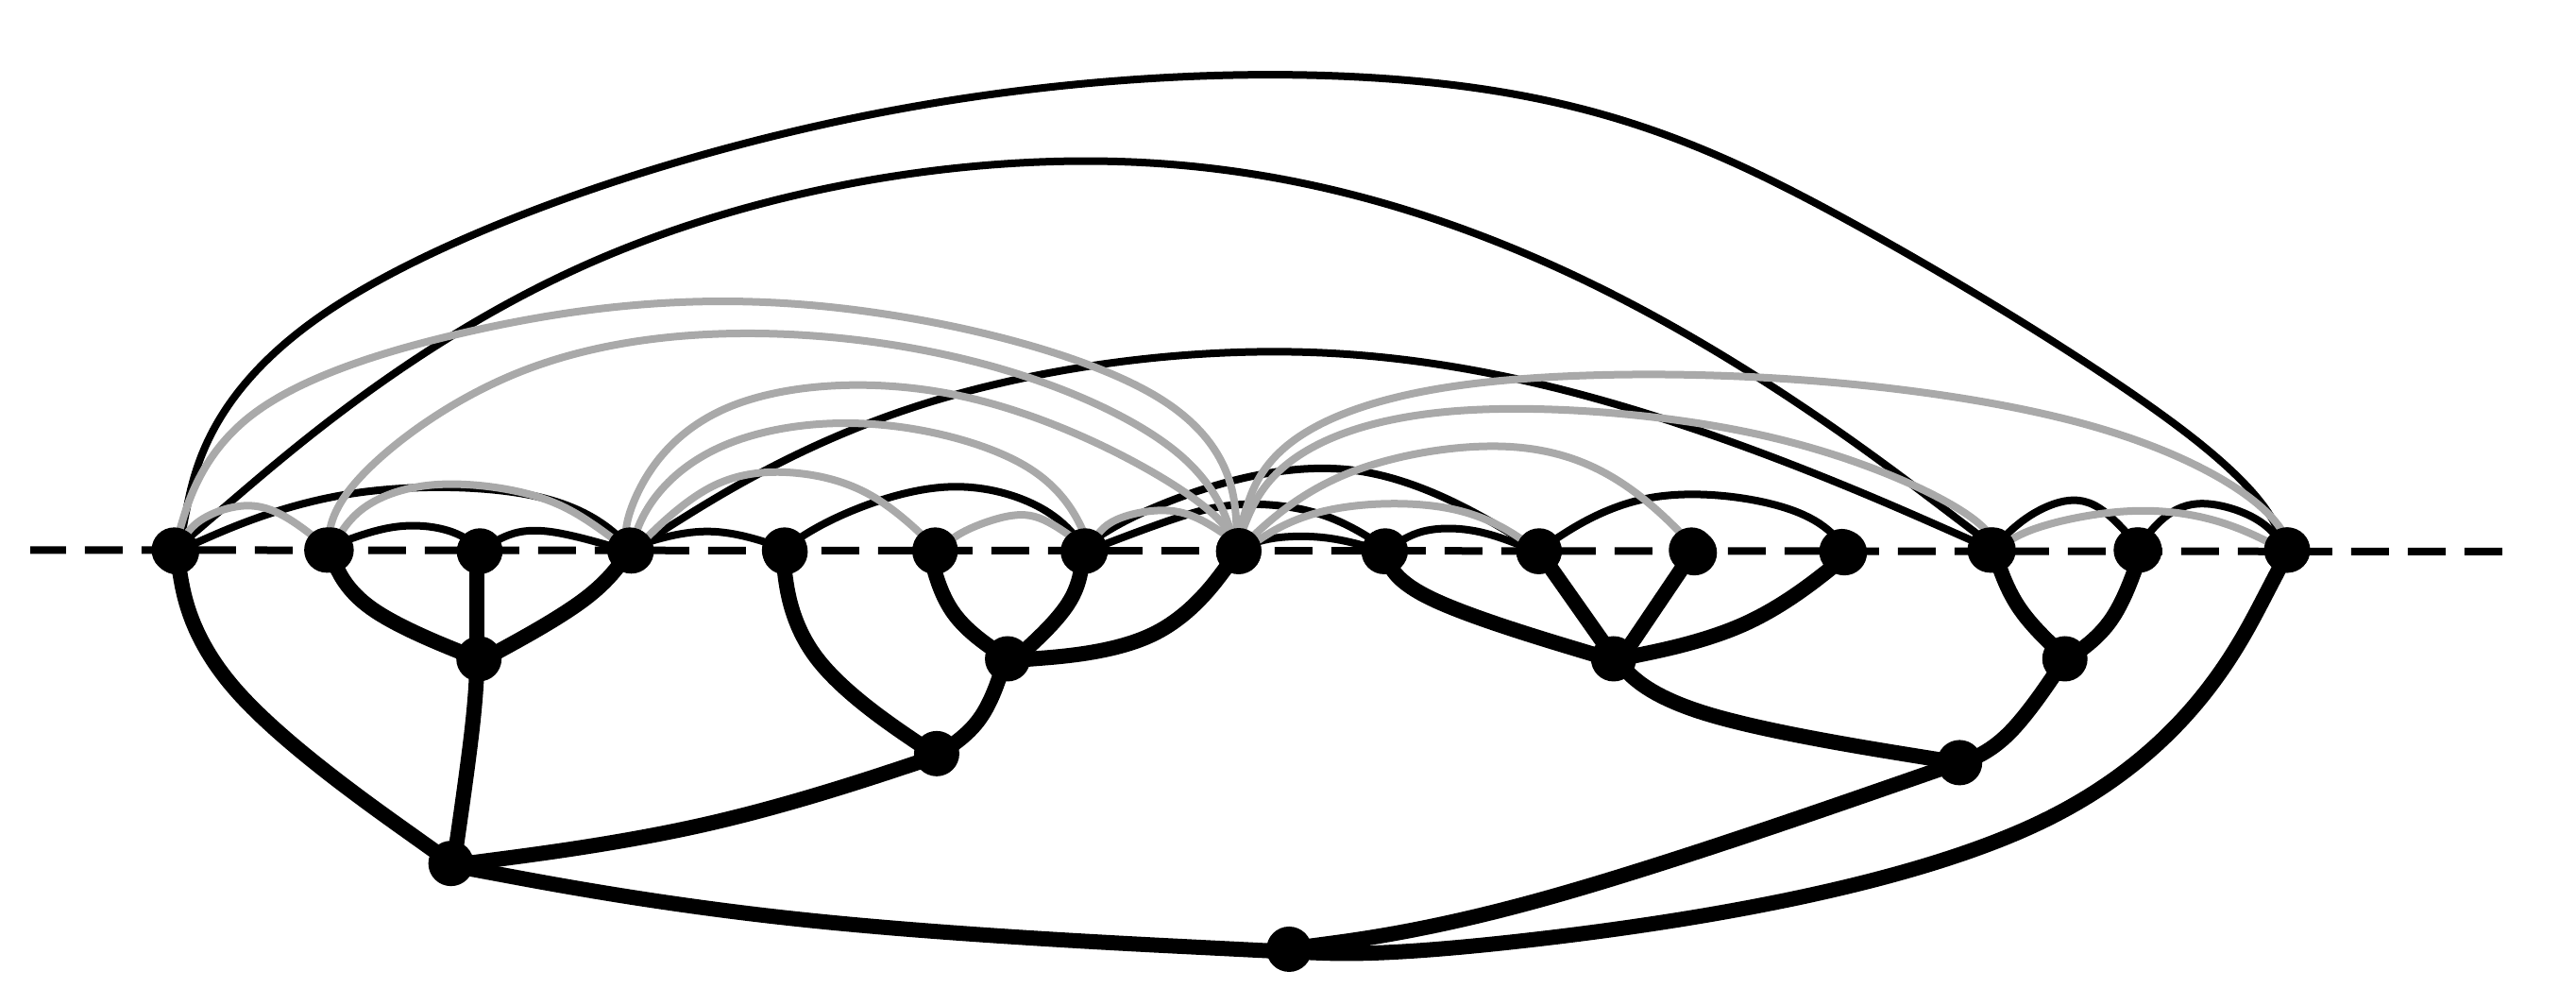
\includegraphics[width=0.8\textwidth]{sefe2}
\end{figure}

Drawing the tree = Restricting permutations by a \PT-tree

\onslide<2>
\vspace{-1em}
\newProb{\probPTree}{\probBook instance $I$ and a \PT-tree~$T$ with leaves~$V$.}{Is there a total order $<\,\in \pi(T)$ solving $I$?}

More structure (same for binary trees):
\newProb{\probQTree}{\probBook instance $I$ and a \Q-tree~$T$ with leaves~$V$.}{Is there a total order $<\,\in \pi(T)$ solving $I$?}
\end{overprint}
\end{frame}

\begin{frame}{Example}

\begin{overprint}

\onslide<1>
\begin{figure}
\centering
\scalebox{1.0}{%
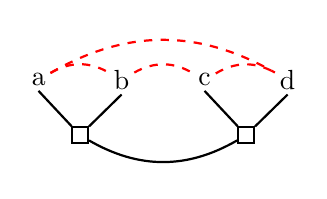
\begin{tikzpicture}
% ab || cd
\begin{scope}
\node (a) {a};
\node[right of=a] (b) {b};
\node[right of=b] (c) {c};
\node[right of=c] (d) {d};

\node[rectangle, draw] (c1) at ($ 0.5*($(a) + (b)$) + (0, -2em) $) {};
\node[rectangle, draw] (c2) at ($ 0.5*($(c) + (d)$) + (0, -2em) $) {};

\draw (c1) edge (a.south);
\draw (c1) edge (b.south);
\draw (c2) edge (c.south);
\draw (c2) edge (d.south);
\draw (c2) edge[bend left] (c1);
\end{scope}

\drawedges[bend left,edge1]{a/b,c/d}
\drawedges[bend left,edge1]{b/c,a/d}
\end{tikzpicture}}
\end{figure}

\begin{itemize}
  \item What happens to the forbidden suborder constraint?
  \item[$\Rightarrow$] 2-CNF formula (Boolean equations) on orientation of \Q-nodes
\end{itemize}

\onslide<2>
\begin{figure}
\centering
\scalebox{1.0}{%
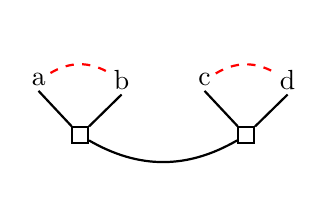
\begin{tikzpicture}
% ab || cd
\begin{scope}
\node (a) {a};
\node[right of=a] (b) {b};
\node[right of=b] (c) {c};
\node[right of=c] (d) {d};

\node[rectangle, draw] (c1) at ($ 0.5*($(a) + (b)$) + (0, -2em) $) {};
\node[rectangle, draw] (c2) at ($ 0.5*($(c) + (d)$) + (0, -2em) $) {};

\draw (c1) edge (a.south);
\draw (c1) edge (b.south);
\draw (c2) edge (c.south);
\draw (c2) edge (d.south);
\draw (c2) edge[bend left] (c1);
\end{scope}

\drawedges[bend left,white]{b/c,a/d}
\drawedges[bend left,edge1]{a/b,c/d}
\end{tikzpicture}}
\end{figure}

\begin{itemize}
\item $\{a, b\}$, $\{c, d\}$: \bool{true}
\end{itemize}
\onslide<3>

\begin{figure}
\centering
\scalebox{0.8}{%
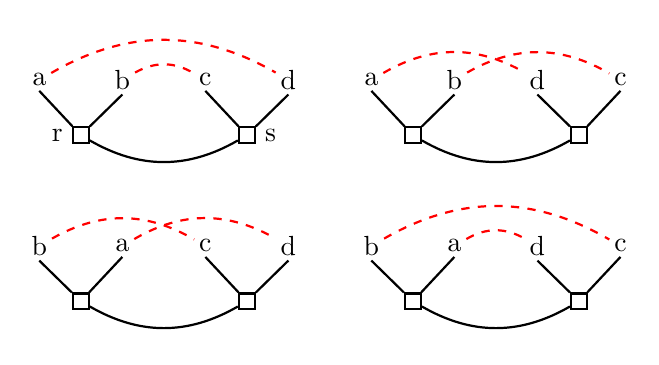
\begin{tikzpicture}
% ab || cd
\begin{scope}
\node (a) {a};
\node[right of=a] (b) {b};
\node[right of=b] (c) {c};
\node[right of=c] (d) {d};

\node[rectangle, draw] (c1) at ($ 0.5*($(a) + (b)$) + (0, -2em) $) {};
\node[rectangle, draw] (c2) at ($ 0.5*($(c) + (d)$) + (0, -2em) $) {};
\node at ($ (c1) + (-.3,0)$) {r};
\node at ($ (c2) + (+.3,0)$) {s};

\draw (c1) edge (a.south);
\draw (c1) edge (b.south);
\draw (c2) edge (c.south);
\draw (c2) edge (d.south);
\draw (c2) edge[bend left] (c1);
\drawedges[bend left,edge1]{b/c,a/d}
\end{scope}

\begin{scope}[xshift=12em]
\node (a) {a};
\node[right of=a] (b) {b};
\node[right of=b] (c) {d};
\node[right of=c] (d) {c};

\node[rectangle, draw] (c1) at ($ 0.5*($(a) + (b)$) + (0, -2em) $) {};
\node[rectangle, draw] (c2) at ($ 0.5*($(c) + (d)$) + (0, -2em) $) {};

\draw (c1) edge (a.south);
\draw (c1) edge (b.south);
\draw (c2) edge (c.south);
\draw (c2) edge (d.south);
\draw (c2) edge[bend left] (c1);
\drawedges[bend left,edge1]{b/d,a/c}
\end{scope}

\begin{scope}[yshift=-6em]
\node (a) {b};
\node[right of=a] (b) {a};
\node[right of=b] (c) {c};
\node[right of=c] (d) {d};

\node[rectangle, draw] (c1) at ($ 0.5*($(a) + (b)$) + (0, -2em) $) {};
\node[rectangle, draw] (c2) at ($ 0.5*($(c) + (d)$) + (0, -2em) $) {};

\draw (c1) edge (a.south);
\draw (c1) edge (b.south);
\draw (c2) edge (c.south);
\draw (c2) edge (d.south);
\draw (c2) edge[bend left] (c1);
\drawedges[bend left,edge1]{a/c,b/d}
\end{scope}

\begin{scope}[yshift=-6em,xshift=12em]
\node (a) {b};
\node[right of=a] (b) {a};
\node[right of=b] (c) {d};
\node[right of=c] (d) {c};

\node[rectangle, draw] (c1) at ($ 0.5*($(a) + (b)$) + (0, -2em) $) {};
\node[rectangle, draw] (c2) at ($ 0.5*($(c) + (d)$) + (0, -2em) $) {};

\draw (c1) edge (a.south);
\draw (c1) edge (b.south);
\draw (c2) edge (c.south);
\draw (c2) edge (d.south);
\draw (c2) edge[bend left] (c1);
\drawedges[bend left,edge1]{b/c,a/d}
\end{scope}

\end{tikzpicture}}
\end{figure}

\begin{itemize}
\item $\{a, d\}$, $\{b, c\}$: $a < b \Leftrightarrow c < d$\\
\item Fix reference orientation of inner nodes~$r$
\item Boolean variable~$o_r$ for being in reference orientation  
\item[$\Rightarrow$] $o_r \Leftrightarrow o_s$
\end{itemize}
\end{overprint}
\end{frame}

%\begin{frame}{Quadratic-time decision}
%%Idea:
%\begin{itemize}
%\item Map to \probTwoSat instance
%\item Fix reference orientation of inner nodes~$r$ of~$T$
%\item Let Boolean variable $o_r$ express~$r$ being in reference orientation
%\item Constraint for two edges yields 2-\CNF formula in constant time
%\end{itemize}
%\end{frame}

%\begin{frame}{Conventions}
%\begin{itemize}
%  \item Let $(V, E_1, \dotsc, E_k)$ be the \probBook instance we consider and $T$~be the \Q-tree on the leaves~$V$ that the vertex order should come from
%  \item For all~$M \subseteq V$ let $r(M)$ be the lowest common ancestor of the vertices~$M$ in~$T$
%  \item Fix a reference orientation for all inner nodes~$r$ of~$T$
%  \item Let the Boolean variable~$o_r$ express~$r$ being in reference orientation 
%\end{itemize}
%\end{frame}

%%%%%%%%%%%%%%%%%%%%%%%%% Book constraints
\begin{frame}{Book constraints to 2-\CNF formula}

\begin{theorem}
\probQTree is solvable in $\OO(kn^2)$ time.
\end{theorem}

\vspace{-.5em}
{
\begin{tabular}{m{0.2\textwidth}m{0.8\textwidth}}


%%% ROW 1
\begin{figure}
\centering
\resizebox{0.2\textwidth}{!}{%
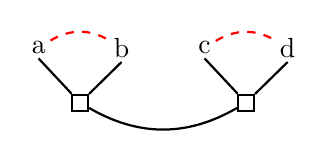
\begin{tikzpicture}
% ab || cd
\begin{scope}
\node (a) {a};
\node[right of=a] (b) {b};
\node[right of=b] (c) {c};
\node[right of=c] (d) {d};

\node[rectangle, draw] (c1) at ($ 0.5*($(a) + (b)$) + (0, -2em) $) {};
\node[rectangle, draw] (c2) at ($ 0.5*($(c) + (d)$) + (0, -2em) $) {};

\draw (c1) edge (a.south);
\draw (c1) edge (b.south);
\draw (c2) edge (c.south);
\draw (c2) edge (d.south);
\draw (c2) edge[bend left] (c1);
\end{scope}
\drawedges[bend left,edge1]{a/b,c/d}
\end{tikzpicture}}
\end{figure} &
\bool{true}\\[-2em]

%%% ROW 2
\begin{figure}
\centering

\resizebox{0.2\textwidth}{!}{%
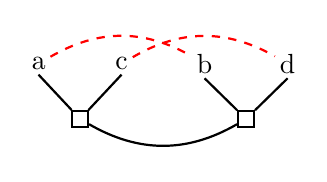
\begin{tikzpicture}

% ac || bd
\begin{scope}[xshift=5cm]
\node (a) {a};
\node[right of=a] (b) {c};
\node[right of=b] (c) {b};
\node[right of=c] (d) {d};

\node[rectangle, draw] (c1) at ($ 0.5*($(a) + (b)$) + (0, -2em) $) {};
\node[rectangle, draw] (c2) at ($ 0.5*($(c) + (d)$) + (0, -2em) $) {};

\draw (c1) edge (a.south);
\draw (c1) edge (b.south);
\draw (c2) edge (c.south);
\draw (c2) edge (d.south);
\draw (c2) edge[bend left] (c1);
\drawedges[bend left,edge1]{a/c,b/d}
\end{scope}

\end{tikzpicture}}
\end{figure}
 
 & \bool{o_{r(a, c)} \Leftrightarrow o_{r(b, d)}} or 
     \bool{o_{r(a, c)} \Leftrightarrow \lnot o_{r(b, d)}} \\[-2em]

%%% ROW 3
  \begin{figure}
  \centering

\resizebox{0.2\textwidth}{!}{%
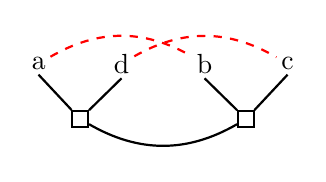
\begin{tikzpicture}
% ad || bc
\begin{scope}[xshift=0cm,yshift=-3cm]
\node (a) {a};
\node[right of=a] (b) {d};
\node[right of=b] (c) {b};
\node[right of=c] (d) {c};

\node[rectangle, draw] (c1) at ($ 0.5*($(a) + (b)$) + (0, -2em) $) {};
\node[rectangle, draw] (c2) at ($ 0.5*($(c) + (d)$) + (0, -2em) $) {};

\draw (c1) edge (a.south);
\draw (c1) edge (b.south);
\draw (c2) edge (c.south);
\draw (c2) edge (d.south);
\draw (c2) edge[bend left] (c1);
\drawedges[bend left,edge1]{a/c,b/d}
\end{scope}
\end{tikzpicture}}
\end{figure} &
     \bool{o_{r(a, d)} \Leftrightarrow o_{r(b, c)}} or
     \bool{o_{r(a, d)} \Leftrightarrow \lnot o_{r(b, c)}}\\[-1.5em]

%%% ROW 4
  \begin{figure}
\centering

\resizebox{0.2\textwidth}{!}{%
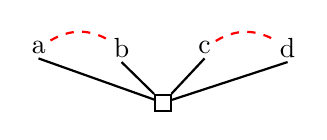
\begin{tikzpicture}
% abcd
\begin{scope}[xshift=5cm,yshift=-3cm]
\node (a) {a};
\node[right of=a] (b) {b};
\node[right of=b] (c) {c};
\node[right of=c] (d) {d};

\node[rectangle, draw] (c1) at ($ 0.5*($(b) + (c)$) + (0, -2em) $) {};

\draw (c1) edge (a.south);
\draw (c1) edge (b.south);
\draw (c1) edge (c.south);
\draw (c1) edge (d.south);
\drawedges[bend left,edge1]{a/b,c/d}
\end{scope}
\end{tikzpicture}} 
\end{figure} & \bool{true} or \bool{false}

\end{tabular}}
\end{frame}
%\section{Multiple spines}

\begin{frame}{Multiple spines}
Take multiple spines:
\tikzsetnextfilename{t_two_spines}
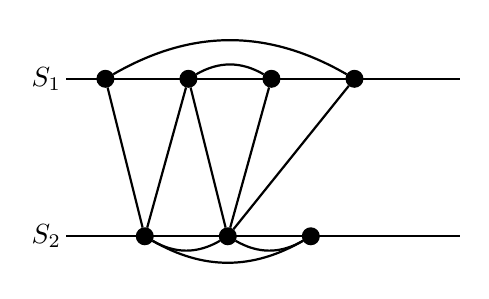
\begin{tikzpicture}

\draw (0, 0) node[left] {$S_2$} -- (5, 0);
\draw (0, 2) node[left] {$S_1$} -- (5, 2);

\tikzstyle{every node}+=[circle,draw,fill]

\node[circle,draw] (o1) at (1, 0) {};
\node[right of=o1] (o2) {};
\node[right of=o2] (o3) {};

\node (u1) at (0.5, 2) {};
\node[right of=u1] (u2) {};
\node[right of=u2] (u3) {};
\node[right of=u3] (u4) {};

\drawedges[bend right]{o1/o2,o1/o3,o2/o3}
\drawedges{o1/u1,o1/u2,o2/u2,o2/u3,o2/u4}
\drawedges[bend left]{u1/u4,u2/u3}

\end{tikzpicture}
%\newProb{\probMul}{Vertex sets~$V_1$, \dots, $V_k$ and
%edge sets $E_0 \subseteq \binom{V_1}{2}$, $E_1 \subseteq V_1\times V_2$,
%\dots, $E_{k-1} \subseteq V_{k-1} \times V_k$, $E_k \subseteq \binom{V_k}{2}$.}{Is there
%a planar drawing of $(V_1 \cup \dotsb \cup V_k, E_0 \cup \dotsb \cup E_k)$ such that
%a vertex in~$V_i$ lies on~$S_i$ for all~$i \in \range{k}$, edges do not cross a spine,
%the edges in~$E_0$ lie completely above~$S_1$ and the edges in~$E_k$ lie completely below~$S_k$?}
Without caps: Solvable in linear time [Jünger et al., 1999].
\end{frame}

\begin{frame}{Level planarity}
Level planarity is an ordering problem:
\begin{figure}[\placement]
\centering

%\resizebox{\textwidth}{!}{
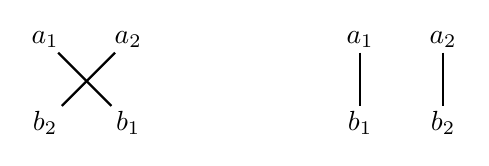
\begin{tikzpicture}

%\tikzstyle{every node}+=[circle,draw]

\node (A1) {$a_1$};
\node[right of=A1] (A2) {$a_2$};
\node[below of=A1] (B2) {$b_2$};
\node[right of=B2] (B1) {$b_1$};
\draw (A1) edge (B1);
\draw (A2) edge (B2);

\begin{scope}[xshift=4cm]
\node (A1) {$a_1$};
\node[right of=A1] (A2) {$a_2$};
\node[below of=A1] (B1) {$b_1$};
\node[right of=B1] (B2) {$b_2$};
\draw (A1) edge (B1);
\draw (A2) edge (B2);
\end{scope}

\end{tikzpicture}
%}
\end{figure}
Forbidden: $a_1 <_i a_2 \land b_2 < b_1$ for $(a_1, b_1), (a_2, b_2) \in E_i$ 
\end{frame}

%\begin{frame}{Observations}
%
%Embeddability only depends on the order of the vertices on the spines:
%\begin{itemize}
%\item Caps come from page embedding
%\item Two edges between TODO
%\end{itemize}
%\end{frame}

\begin{frame}{Mapping to 2-page \probPTree}

\begin{theorem}
A \probMul instance is equivalent to a special 2-page \probPTree instance.
\end{theorem}

\begin{figure}[\placement]
\centering

\resizebox{0.90\textwidth}{!}{
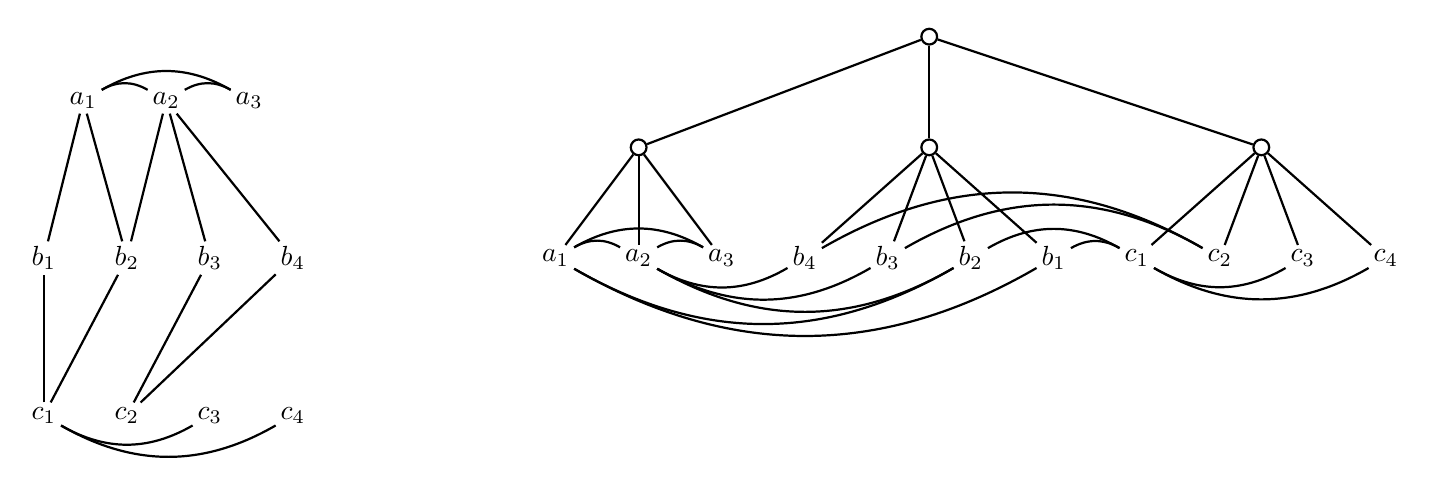
\begin{tikzpicture}

%\draw (0, 0) node[left] {} -- (5, 0);
%\draw (0, -2) node[left] {} -- (5, -2);

%\tikzstyle{every node}+=[circle,draw,fill]

\node (a1) at (1, 0) {$a_1$};
\node[right of=a1] (a2) {$a_2$};
\node[right of=a2] (a3) {$a_3$};

\node (b1) at (0.5, -2) {$b_1$};
\node[right of=b1] (b2) {$b_2$};
\node[right of=b2] (b3) {$b_3$};
\node[right of=b3] (b4) {$b_4$};

\node (c1) at (0.5, -4) {$c_1$};
\node[right of=c1] (c2) {$c_2$};
\node[right of=c2] (c3) {$c_3$};
\node[right of=c3] (c4) {$c_4$};


\drawedges[bend left]{a1/a2,a1/a3,a2/a3}
\drawedges{a1/b1,a1/b2,a2/b2,a2/b3,a2/b4}
\drawedges{c1/b1,c1/b2,c2/b3,c2/b4}
\drawedges[bend right]{c1/c4,c1/c3}

\node[draw=none,fill=none] at (5.5,-2) {{\Huge $\rightsquigarrow$}};

\begin{scope}[xshift=7cm,yshift=-2cm]

%\draw (-1, 0) -- (9, 0);

\node (a1) at (0, 0) {$a_1$};
\node[right of=a1] (a2) {$a_2$};
\node[right of=a2] (a3) {$a_3$};

\node[right of=a3] (b4) {$b_4$};
\node[right of=b4] (b3) {$b_3$};
\node[right of=b3] (b2) {$b_2$};
\node[right of=b2] (b1) {$b_1$};

\node[right of=b1] (c1) {$c_1$};
\node[right of=c1] (c2) {$c_2$};
\node[right of=c2] (c3) {$c_3$};
\node[right of=c3] (c4) {$c_4$};

\drawedges[bend left]{a1/a2,a1/a3,a2/a3}
\drawedges[bend right]{a1/b1,a1/b2,a2/b2,a2/b3,a2/b4}
\drawedges[bend right]{c1/b1,c1/b2,c2/b3,c2/b4}
\drawedges[bend right]{c1/c4,c1/c3}

\end{scope}

\visible<2->{
\node[circle, draw] (r1) at ($ (a2) + (0, 4em) $) {};
\node[circle, draw] (r2) at ($ 0.5*($ (b2) + (b3) $) + (0, 4em)$) {};
\node[circle, draw] (r3) at ($ 0.5*($ (c2) + (c3) $) + (0, 4em)$) {};
\node[circle, draw] (r) at ($ (r2) + (0, 4em) $) {};
\drawedges[ultra thick]{r1/a1,r1/a2,r1/a3,r2/b1,r2/b2,r2/b3,r2/b4,r3/c1,r3/c2,r3/c3,r3/c4,r/r1,r/r2,r/r3}
}

\end{tikzpicture}
}
\end{figure}

\end{frame}

\miniframesoff

%\begin{frame}{The end}
%
%\begin{center}
%\large{Thank you for your attention.}
%\end{center}
%
%\vfill
%\small{I would also like to thank my advisors Dipl.-Inform. Thomas Bläsius and
%Dr. Ignaz Rutter for all their continued support, guidance, advice as well
%as for the insightful discussions I had with them.}
%
%\end{frame} 

\begin{frame}{Conclusion and outlook}
\begin{overprint}
\onslide<1>\solutionTri{1}{0.6\textwidth}
\onslide<2>\solutionTri{2}{0.6\textwidth}
\onslide<3>\solutionTri{3}{0.6\textwidth}
\onslide<4>\solutionTri{4}{0.6\textwidth}
\onslide<5>\solutionTri{5}{0.6\textwidth}
\onslide<6>\solutionTri{6}{0.6\textwidth}
\vspace{-1.8em}
\begin{itemize}
  \item Complexity for constant number of pages?
  \item Complexity when constrained by a \PT-tree?
\end{itemize}

\end{overprint}
\end{frame}

\begin{frame}{Addendum: Multiple spines}
\begin{figure}[\placement]
\centering

\resizebox{0.90\textwidth}{!}{
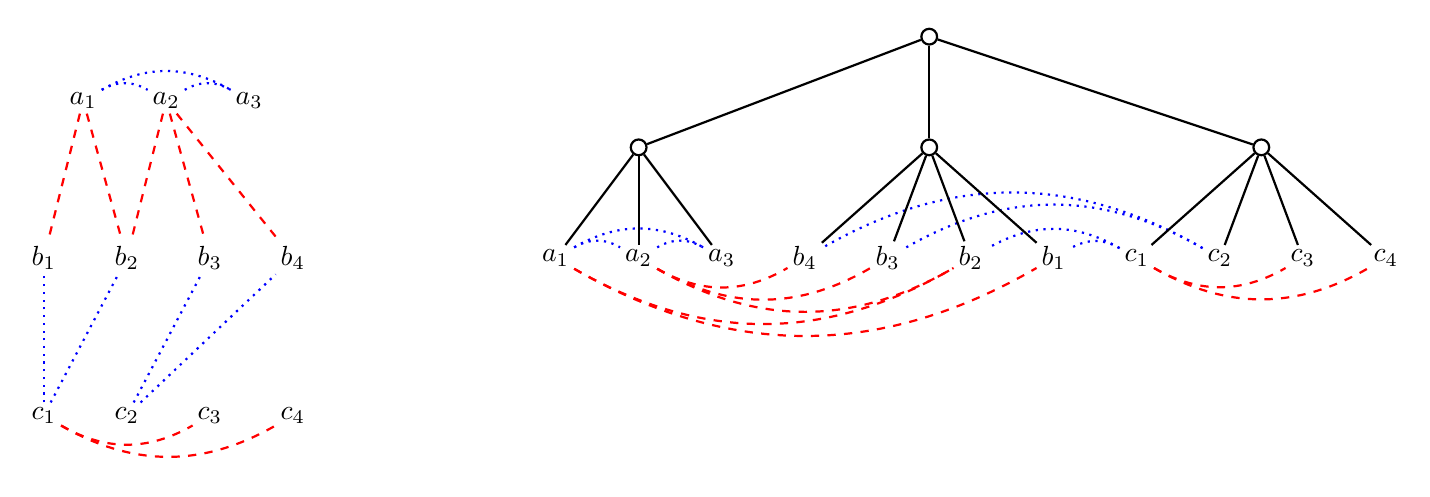
\begin{tikzpicture}

%\draw (0, 0) node[left] {} -- (5, 0);
%\draw (0, -2) node[left] {} -- (5, -2);

%\tikzstyle{every node}+=[circle,draw,fill]

\node (a1) at (1, 0) {$a_1$};
\node[right of=a1] (a2) {$a_2$};
\node[right of=a2] (a3) {$a_3$};

\node (b1) at (0.5, -2) {$b_1$};
\node[right of=b1] (b2) {$b_2$};
\node[right of=b2] (b3) {$b_3$};
\node[right of=b3] (b4) {$b_4$};

\node (c1) at (0.5, -4) {$c_1$};
\node[right of=c1] (c2) {$c_2$};
\node[right of=c2] (c3) {$c_3$};
\node[right of=c3] (c4) {$c_4$};


\drawedges[bend left,edge2]{a1/a2,a1/a3,a2/a3}
\drawedges[edge1]{a1/b1,a1/b2,a2/b2,a2/b3,a2/b4}
\drawedges[edge2]{c1/b1,c1/b2,c2/b3,c2/b4}
\drawedges[bend right,edge1]{c1/c4,c1/c3}

\node[draw=none,fill=none] at (5.5,-2) {{\Huge $\rightsquigarrow$}};

\begin{scope}[xshift=7cm,yshift=-2cm]

%\draw (-1, 0) -- (9, 0);

\node (a1) at (0, 0) {$a_1$};
\node[right of=a1] (a2) {$a_2$};
\node[right of=a2] (a3) {$a_3$};

\node[right of=a3] (b4) {$b_4$};
\node[right of=b4] (b3) {$b_3$};
\node[right of=b3] (b2) {$b_2$};
\node[right of=b2] (b1) {$b_1$};

\node[right of=b1] (c1) {$c_1$};
\node[right of=c1] (c2) {$c_2$};
\node[right of=c2] (c3) {$c_3$};
\node[right of=c3] (c4) {$c_4$};

\drawedges[bend left,edge2]{a1/a2,a1/a3,a2/a3}
\drawedges[bend right,edge1]{a1/b1,a1/b2,a2/b2,a2/b3,a2/b4}
\drawedges[bend right,edge2]{c1/b1,c1/b2,c2/b3,c2/b4}
\drawedges[bend right,edge1]{c1/c4,c1/c3}

\end{scope}

\node[circle, draw] (r1) at ($ (a2) + (0, 4em) $) {};
\node[circle, draw] (r2) at ($ 0.5*($ (b2) + (b3) $) + (0, 4em)$) {};
\node[circle, draw] (r3) at ($ 0.5*($ (c2) + (c3) $) + (0, 4em)$) {};
\node[circle, draw] (r) at ($ (r2) + (0, 4em) $) {};
\drawedges[ultra thick]{r1/a1,r1/a2,r1/a3,r2/b1,r2/b2,r2/b3,r2/b4,r3/c1,r3/c2,r3/c3,r3/c4,r/r1,r/r2,r/r3}

\end{tikzpicture}
}
\end{figure}
\end{frame}

\end{document}
